% Szglab4
% ===========================================================================
%
\chapter{Grafikus felület specifikációja}

\thispagestyle{fancy}

\section{A grafikus interfész}
\comment{A menürendszer, a kezelői felület grafikus képe. A grafikus felület megjelenését, a használt ikonokat, stb screenshot-szerű képekkel kell bemutatni. Az építészetben ez a homlokzati terv.}

A játék indításakor az alábbi menü jön be:

\begin{figure}[H]
	\begin{center}
		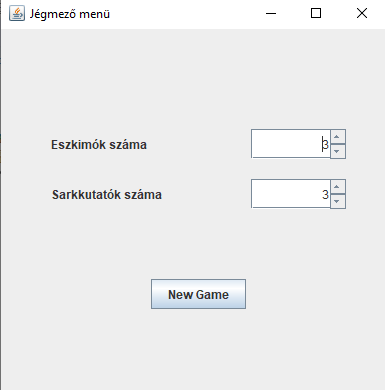
\includegraphics[width=11cm]{chapters/chapter11/res/menu.png}
		\caption{A játék menüjét bemutató ábra}
		\label{fig:Menu}
	\end{center}
\end{figure}

A két Spinner segítségével kiválasztható a játékosok száma, kutatókra és eszkimókra lebontva.
A New Game gomb segítségével indítható el a játék, ami működés közben valahogy így néz ki:

\begin{figure}[H]
	\begin{center}
		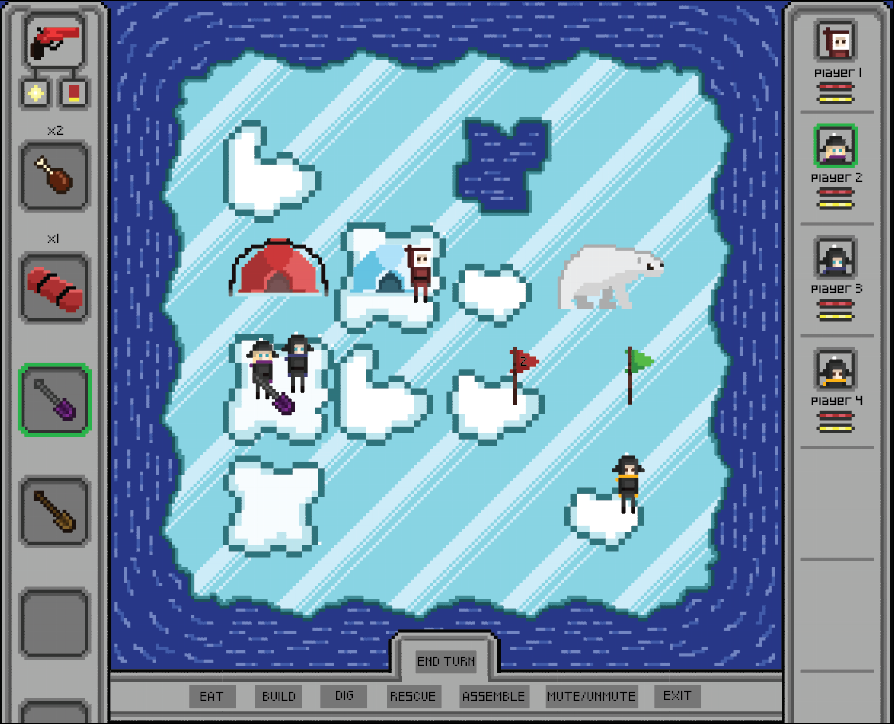
\includegraphics[width=11cm]{chapters/chapter11/res/game1.png}
		\caption{Kép a játékról, eszközökkel}
		\label{fig:Game1}
	\end{center}
\end{figure}
\begin{figure}[H]
	\begin{center}
		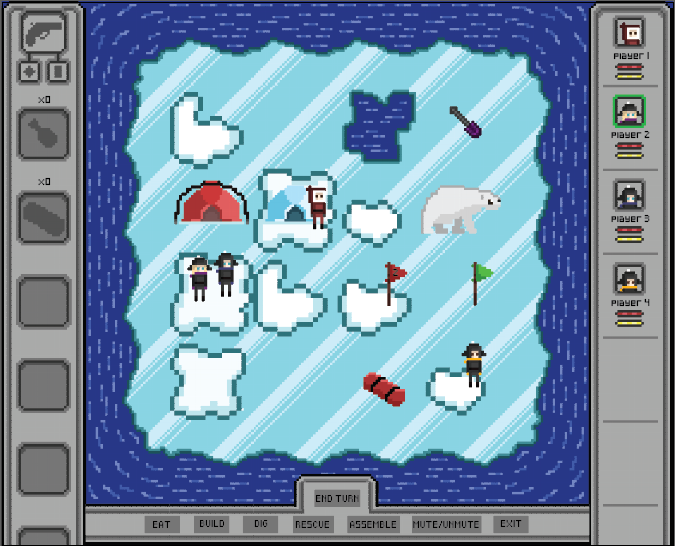
\includegraphics[width=11cm]{chapters/chapter11/res/game2.png}
		\caption{Kép a játékról, eszközök nélkül}
		\label{fig:Game2}
	\end{center}
\end{figure}

A képen láthatók a játékosok jobb oldalt, akik részt vesznek a játékban. Az ikonjuk alapján megkülönböztethetőek egyértelműen. Az ikon alatt pirossal a testhő, sárgával a játékos energiája látható.
Az aktuálisan kiválasztott játékost, akit zöld keret vesz körül, lehet irányítani, és láthatóak a tárgyai a bal oldalon. Az éppen használatban lévő tárgyakat szintén zöld keret veszi körül. Az élelem és sátorzacskó fogyócikkek fölött számláló helyezkedik el, ami a kiválasztott játékosnak éppen birtokában lévő mennyiséget jelzi belőlük. A tárgyak között látható törékeny falapát, míg törhetetlen lila kristálylapát is.
A képernyő alján az akciógombok helyezkednek el, ezekkel lehet a modellben specifikált use-casek szerint irányítani az éppen kiválasztott játékost. Emellett ha már nem szeretne akciót végezni, véget vethet körének a játékos. A játékból való kilépés és a hang kikapcsolása is ezen a gombsoron kapott helyet.
A képernyő közepén található a lényeg, maga a játék megjelenítése. A jégmezőt a hideg, fagyos óceán veszi körül, míg a tükörsima jégen félelmetes jegesmedve szörny, és tőle rettegő, onnan menekülni vágyó játékosok láthatók. Kapucniban az iglulakó eszkimók találhatók, míg sapkában a sarkkutatók fedezik fel a jégtáblák rejtelmeit. Felfedezett jégtábláik teherbírását zászlóval jelölik: zölddel, ha az nem törhet el, míg pirossal és egy számmal, ha az eltörhet a számot meghaladó játékosok lába alatt.
A jégen találhatók tárgyak is, sátorzacskó, törhetetlen lapát, emellett vannak épületek is lerakva, iglu és sátor is.
A jégmezőn található hóval nem fedett vizesgödör, hóval fedett és sima jégtábla is. A hómennyiség az üres jégtől kezdve 5 réteg hóig terjedhet, mindegyik látható a pillanatképünkön.
A jégmezőn néha feltámad a hóvihar, ez az alábbihoz hasonló animációval lesz majd megjelenítve:

\begin{figure}[H]
	\begin{center}
		
\includegraphics[width=11cm]{chapters/chapter11/res/storm.png}
		\caption{Kép a játékban a hóviharról}
		\label{fig:Snowstorm}
	\end{center}
\end{figure}

\section{A grafikus rendszer architektúrája}
\comment{A felület működésének elve, a grafikus rendszer architektúrája (struktúra diagramok). A struktúra diagramokon a prototípus azon és csak azon osztályainak is szerepelnie kell, amelyekhez a grafikus felületet létrehozó osztályok kapcsolódnak.}

\subsection{A felület működési elve}
\comment{Le kell írni, hogy a grafikai megjelenésért felelős osztályok, objektumok hogyan kapcsolódnak a meglevő rendszerhez, a megjelenítés során mi volt az alapelv. Törekedni kell az MVC megvalósításra. Alapelvek lehetnek: \textbf{push} alapú: a modell értesíti a felületet, hogy változott; \textbf{pull} alapú: a felület kérdezi le a modellt, hogy változott-e; \textbf{kevert}: a kettő kombinációja.}

\subsection{A felület osztály-struktúrája}
\comment{Osztálydiagram. Minden új osztály, és azon régiek, akik az újakhoz közvetlenül kapcsolódnak.}

\section{A grafikus objektumok felsorolása}
\comment{Az új osztályok felsorolása. Az régi osztályok közül azoknak a felsorolása, ahol változás volt. Ezek esetén csak a változásokat kell leírni.}

\subsection{Osztály1}
\begin{itemize}
\item Felelősség\newline
\comment{Mi az osztály felelőssége. Kb 1 bekezdés. Ha szükséges, akkor state-chart is.}
\item Ősosztályok\newline
\comment{Mely osztályokból származik (öröklési hierarchia)\newline
Legősebb osztály $\rightarrow$ Ősosztály2 $\rightarrow$ Ősosztály3...}
\item Interfészek\newline
\comment{Mely interfészeket valósítja meg.}
\item Attribútumok\newline
\comment{Milyen attribútumai vannak}
	\begin{itemize}
		\item attribútum1: attribútum jellemzése: mire való, láthatósága (UML jelöléssel), típusa
		\item attribútum2: attribútum jellemzése: mire való, láthatósága (UML jelöléssel), típusa
	\end{itemize}
\item Metódusok\newline
\comment{Milyen publikus, protected és privát  metódusokkal rendelkezik. Metódusonként precíz leírás, ha szükséges, activity diagram is  a metódusban megvalósítandó algoritmusról.}
	\begin{itemize}
		\item int foo(Osztály3 o1, Osztály4 o2): metódus leírása, láthatósága (UML jelöléssel)
		\item int bar(Osztály5 o1): metódus leírása, láthatósága (UML jelöléssel)
	\end{itemize}
\end{itemize}

\subsection{Osztály2}
\begin{itemize}
\item Felelősség\newline
\comment{Mi az osztály felelőssége. Kb 1 bekezdés. Ha szükséges, akkor state-chart is.}
\item Ősosztályok\newline
\comment{Mely osztályokból származik (öröklési hierarchia)\newline
Legősebb osztály $\rightarrow$ Ősosztály2 $\rightarrow$ Ősosztály3...}
\item Interfészek\newline
\comment{Mely interfészeket valósítja meg.}
\item Attribútumok\newline
\comment{Milyen attribútumai vannak}
	\begin{itemize}
		\item attribútum1: attribútum jellemzése: mire való, láthatósága (UML jelöléssel), típusa
		\item attribútum2: attribútum jellemzése: mire való, láthatósága (UML jelöléssel), típusa
	\end{itemize}
\item Metódusok\newline
\comment{Milyen publikus, protected és privát  metódusokkal rendelkezik. Metódusonként precíz leírás, ha szükséges, activity diagram is  a metódusban megvalósítandó algoritmusról.}
	\begin{itemize}
		\item int foo(Osztály3 o1, Osztály4 o2): metódus leírása, láthatósága (UML jelöléssel)
		\item int bar(Osztály5 o1): metódus leírása, láthatósága (UML jelöléssel)
	\end{itemize}
\end{itemize}

\section{Kapcsolat az alkalmazói rendszerrel}
\comment{Szekvencia-diagramokon ábrázolni kell a grafikus rendszer működését. Konzisztens kell legyen az előző alfejezetekkel. Minden metódus, ami ott szerepel, fel kell tűnjön valamelyik szekvenciában. Minden metódusnak, ami szekvenciában szerepel, szereplnie kell a valamelyik osztálydiagramon.}

